% !TEX root = HW4.tex
\ifthenelse{\equal{\type}{booklet}}{
% !TEX root = HW4.tex
\newcommand{\spEighteenSvmOneA}{\\
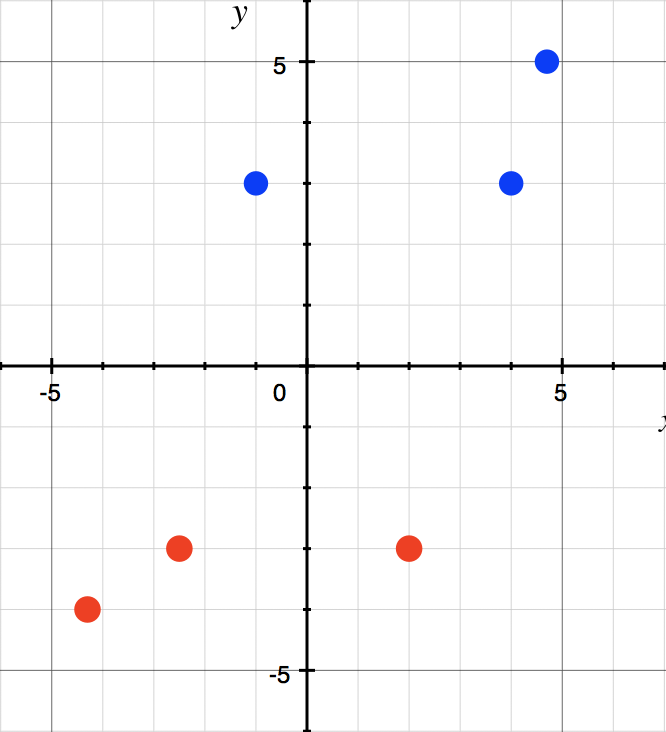
\includegraphics[width=4cm]{1a.png}\\
$\mathbf{w} = [0;\frac{1}{3}]$, $b=0$\\

From the graph its quite clear the $\mathbf{x}_1$ has no effect on the classification. This leaves $\mathbf{w}_2$ and $b$ unknown. We can use the four support vectors to determine the optimal values for these two parameters. We want the decision hyper-plane to be equidistant from each of these vectors which leaves us with $\mathbf{w}_2 = 1$ and $b=0$. $\mathbf{w}_2$ can be further minimized down to $\mathbf{w}_2 = \frac{1}{3}$ to reduce the total cost while conforming the hard SVM constraint. Its important to note that increasing $b$ off of $0$ in either direction requires $\mathbf{w}_2$ to also increase, thereby increasing the total cost. Ex. if $b=\frac{1}{2}$, $\mathbf{w}_2$ would have to be increased to $\frac{1}{2}$, increasing the total cost as mentioned.
}

\newcommand{\spEighteenSvmOneB}{
The support vector are examples: 1, 2, 3, and 5
}

\newcommand{\spEighteenSvmOneC}{
$$
\mathbf{z}=
\begin{bmatrix}
\mathbf{w}_1\\
\mathbf{w}_2\\
b
\end{bmatrix}
P=
\begin{bmatrix}
1 & 0 & 0 \\
0 & 1 & 0 \\
0 & 0 & 0 \\
\end{bmatrix}
\mathbf{q}=
\begin{bmatrix}
0\\
0\\
0
\end{bmatrix}
G=
\begin{bmatrix}
1 & -3 & -1\\
-2.5 & -3 & 1\\
2 & -3 & 1\\
-4.7 & -5 & -1\\
-4 & -3 & -1\\
-4.3 & -4 & 1\\
\end{bmatrix}
\mathbf{h}=
\begin{bmatrix}
-1\\
-1\\
-1\\
-1\\
-1\\
-1\\
\end{bmatrix}
$$
}

\newcommand{\spEighteenSvmOneD}{
When $C=0$ the soft-SVM becomes a hard-SVM and has a margin of 1. If $C=\infty$ the margin is reduced to 0 in order to lower the cost as much as possible.
}

\newcommand{\spEighteenSvmTwoA}{
\begin{align*}
\alpha K_1(\mathbf{x},\mathbf{z}) + \beta K_2(\mathbf{x},\mathbf{z})&=\alpha\Phi(\mathbf{x})^T\Phi(\mathbf{z})+\beta\Phi(\mathbf{x})^T\Phi(\mathbf{z})\\
&=\begin{bmatrix}
\alpha\Phi(\mathbf{x})^T & \beta\Phi(\mathbf{x})^T\\
\end{bmatrix}
\begin{bmatrix}
\alpha\Phi(\mathbf{z}) \\
\beta\Phi(\mathbf{z})
\end{bmatrix} \\
&=(\alpha K_1 + \beta K_2)(\mathbf{x},\mathbf{z}) \\
&=K_3(\mathbf{x},\mathbf{z})
\end{align*}
Which forms a valid kernel function, as the key restriction is that the kernel function must form a proper inner product.
}

\newcommand{\spEighteenSvmTwoB}{
\begin{align*}
K(\mathbf{x},\mathbf{z})
&= (\mathbf{x}^T\mathbf{z})^2 \\
&= (\mathbf{x}_1 \mathbf{z}_1 + \mathbf{x}_2 \mathbf{z}_2)^2 \\
&= (\mathbf{x}_1 \mathbf{z}_1)^2 + 2(\mathbf{x}_1 \mathbf{z}_1)(\mathbf{x}_2 \mathbf{z}_2) + (\mathbf{x}_2 \mathbf{z}_2)^2 \\
&= \mathbf{x}_1^2\mathbf{z}_1^2 + 2\mathbf{x}_1\mathbf{z}_1\mathbf{x}_2\mathbf{z}_2 + \mathbf{x}_2^2\mathbf{z}_2^2 \\
&= \begin{bmatrix}
\mathbf{x}_1^2\\
\sqrt{2}\mathbf{x}_1\mathbf{x}_1\\
\mathbf{x}_2^2\\
\end{bmatrix}^T
\begin{bmatrix}
\mathbf{z}_1^2\\
\sqrt{2}\mathbf{z}_1\mathbf{z}_1\\
\mathbf{z}_2^2\\
\end{bmatrix}\\
\end{align*}

$$
\Phi(\mathbf{x}) = 
\begin{bmatrix}
\mathbf{x}_1^2\\
\sqrt{2}\mathbf{x}_1\mathbf{x}_1\\
\mathbf{x}_2^2\\
\end{bmatrix}
$$
} %The students have to fill this file to print the solution
}{
\input{sp2018_svm_OurSolution} %This file will not be provided to students since it contains the solution
}

% Problem Explanation:
% - first argument is the number of points
% - second argument is the title and the text
\examproblem{10}{SVM Basics\\
Consider the following dataset $\cD$ in the two-dimensional space; $\bx^{(i)} \in \mathbb{R}^2$ and $y^{(i)} \in \{1, -1\}$
\begin{table}	[h]
\centering
\begin{tabular}{|c|c|c|c|}
\hline
$i$ & $\bx_1^{(i)}$ & $\bx_2^{(i)}$ & $y^{(i)}$\\
\hline
1 & -1 & 3& 1\\
2 &  -2.5 & -3 & -1 \\
3 & 2 & -3& -1\\
4 & 4.7 & 5& 1\\
5 & 4 & 3 & 1\\
6 & -4.3& -4& -1 \\
\hline
\end{tabular}
\end{table}
}

Recall a hard SVM is as follows:
\begin{align}\label{eq:svm}
\min\limits_{w, b} \frac{1}{2} \norm{\bw}^2 \;\;\;
\text{s.t.} \;\; y^{(i)}(\bw^\intercal\bx^{(i)} + b \geq 1) \;\; ,\forall (x^{(i)}, y^{(i)}) \in \cD
\end{align} 

%%%%%%%%%%%%%%%%%%%%%%%%%%%%%%%%%%%%%%
%%%%%  BEGINNING OF SUBPROBLEMS LIST
\begin{enumerate}

% Subproblem description
\examproblempart{What is the optimal $\bw$ and $b$? Show all your work and reasoning. (Hint: Draw it out.)
\\}
% Solution box
\framebox[14.7cm][l]{
\begin{minipage}[b]{14.4cm}

\inbooklet{Your answer:
\spEighteenSvmOneA
}

\solution{\spEighteenSvmOneA}
\end{minipage}
}

\examproblempart{Which of the examples are support vectors?\\}
% Solution box
\framebox[14.7cm][l]{
\begin{minipage}[b]{14.4cm}

\inbooklet{Your answer:
\spEighteenSvmOneB
}

\solution{\spEighteenSvmOneB}
\end{minipage}
}

\examproblempart{A standard quadratic program is as follows,
\begin{equation*}
\begin{aligned}
& \underset{\bz}{\text{minimize}}
& \frac{1}{2} \bz^{\intercal}P\bz + \mathbf{q}^{\intercal} \mathbf{z} \\
& \text{subject to}
& G\bz \leq \mathbf{h}
\end{aligned}
\end{equation*}
Rewrite Equation \eqref{eq:svm} into the above form. (\ie define $\bz, P, \mathbf{q}, G, \mathbf{h}$  using $\bw, b$ and values in $\cD$). Write the constraints in the {\bf same order} as provided in $\cD$ and typeset it using \texttt{bmatrix}.\\
}

\framebox[14.7cm][l]{
\begin{minipage}[b]{14.4cm}

\inbooklet{Your answer:
\spEighteenSvmOneC
}

\solution{\spEighteenSvmOneC}
\end{minipage}

}

\examproblempart{Recall that for a soft-SVM we solve the following optimization problem.
\begin{center}
\begin{align}
\min\limits_{w, b} \frac{1}{2} \norm{\bw}^2 + C \cdot \sum\limits_{i=1}^{|D|} \xi^{(i)} \;\;\;
\text{s.t.} \;\; y^{(i)}(\bw^\intercal\bx^{(i)} + b \geq 1 - \xi^{(i)}), \xi^{(i)}\geq 0 \;\; ,\forall (x^{(i)}, y^{(i)}) \in \cD
\end{align} 
\end{center}
Describe what happens to the margin when $C = \infty$ and $C = 0$.
}

\framebox[14.7cm][l]{
\begin{minipage}[b]{14.4cm}

\inbooklet{Your answer:
\spEighteenSvmOneD
}

\solution{\spEighteenSvmOneD}
\end{minipage}

}

%%%%%%%%%%%% END OF SUBPROBLEMS LIST

\end{enumerate}

\examproblem{4}{Kernels\\
\begin{enumerate}
\examproblempart{If $K_1(\bx, \bz)$ and $K_2(\bx, \bz)$ are both valid kernel functions, and $\alpha$ and $\beta$ are positive,
prove that 
\[\alpha K_1(\bx, \bz) + \beta K_2(\bx, \bz)
\]
is also a valid kernel function.
\\}
\framebox[14.7cm][l]{
\begin{minipage}[b]{14.4cm}

\inbooklet{Your answer:
\spEighteenSvmTwoA
}

\solution{\spEighteenSvmTwoA}
\end{minipage}

}

\examproblempart{Show that $K(\bx,\bz) = (\bx^{\intercal}\bz)^2$ is a valid kernel, for $\bx, \bz \in \mathbb{R}^2$.\\ (\ie 
write out the $\Phi(\cdot)$, such that $K(\bx,\bz) = \Phi(\bx)^\intercal\Phi(\bz)$\\}
\framebox[14.7cm][l]{
\begin{minipage}[b]{14.4cm}

\inbooklet{Your answer:
\spEighteenSvmTwoB
}

\solution{\spEighteenSvmTwoB}
\end{minipage}

}

\end{enumerate}
}